\documentclass[11pt,letterpaper]{article}
\usepackage[lmargin=1in,rmargin=1in,tmargin=1in,bmargin=1in]{geometry}
\usepackage{../style/homework}
\usepackage{../style/commands}
\setbool{quotetype}{false} % True: Side; False: Under
\setbool{hideans}{true} % Student: True; Instructor: False

% -------------------
% Content
% -------------------
\begin{document}

\homework{4: Due 05/31}{Nothing has such power to broaden the mind as the ability to investigate systematically and truly all that comes under thy observation in life.}{Marcus Aurelius}

% Problem 
\problem{10} Determine if the relations $f(x)$ and $g(x)$ shown below are functions. Explain why or why not. If the relation is a function, determine its domain, codomain, and range. 
	\[
	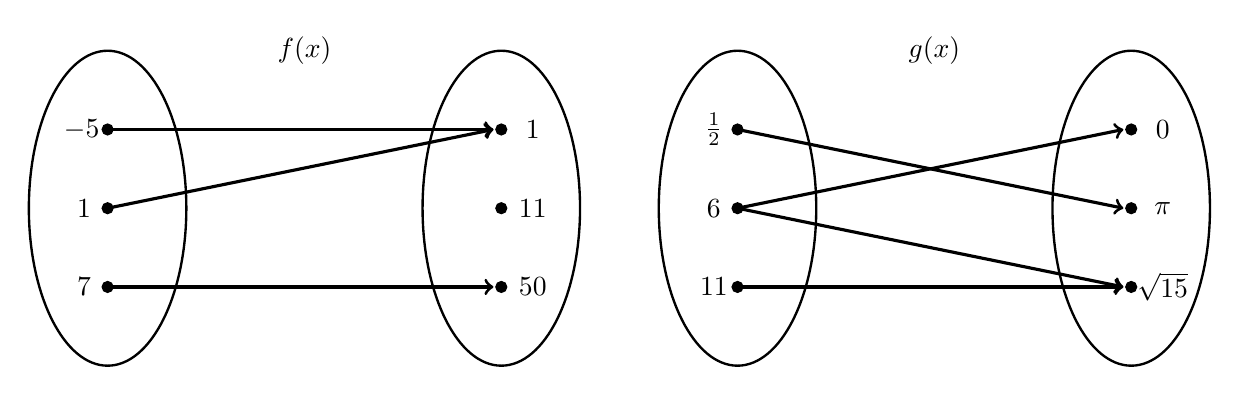
\begin{tikzpicture}
	\node at (2.5,2) {$f(x)$};
	% Ellipses
	\draw[line width=0.03cm] (0,0) circle (1 and 2);
	\draw[line width=0.03cm] (5,0) circle (1 and 2);
	
	% Nodes
	\draw[fill=black] (0,1) circle (0.07);
	\draw[fill=black] (0,0) circle (0.07);
	\draw[fill=black] (0,-1) circle (0.07);
	
	\draw[fill=black] (5,1) circle (0.07);
	\draw[fill=black] (5,0) circle (0.07);
	\draw[fill=black] (5,-1) circle (0.07);
	
	% Arrow
	\draw[line width=0.04cm,->] (0,1) -- (4.9,1);
	\draw[line width=0.04cm,->] (0,0) -- (4.9,1);
	\draw[line width=0.04cm,->] (0,-1) -- (4.9,-1);
	
	% Labels
	\node at (-0.3,1) {$\!-5$};
	\node at (-0.3,0) {$1$};
	\node at (-0.3,-1) {$7$};
	
	\node at (5.4,1) {$1$};
	\node at (5.4,0) {$11$};
	\node at (5.4,-1) {$50$};
	
	\tikzset{shift={(8,0)}}
	%
	\node at (2.5,2) {$g(x)$};
	% Ellipses
	\draw[line width=0.03cm] (0,0) circle (1 and 2);
	\draw[line width=0.03cm] (5,0) circle (1 and 2);
	
	% Nodes
	\draw[fill=black] (0,1) circle (0.07);
	\draw[fill=black] (0,0) circle (0.07);
	\draw[fill=black] (0,-1) circle (0.07);
	
	\draw[fill=black] (5,1) circle (0.07);
	\draw[fill=black] (5,0) circle (0.07);
	\draw[fill=black] (5,-1) circle (0.07);
	
	% Arrow
	\draw[line width=0.04cm,->] (0,1) -- (4.9,0);
	\draw[line width=0.04cm,->] (0,0) -- (4.9,1);
	\draw[line width=0.04cm,->] (0,0) -- (4.9,-1);
	\draw[line width=0.04cm,->] (0,-1) -- (4.9,-1);
	
	% Labels
	\node at (-0.3,1) {$\frac{1}{2}$};
	\node at (-0.3,0) {$6$};
	\node at (-0.3,-1) {$11$};
	
	\node at (5.4,1) {$0$};
	\node at (5.4,0) {$\pi$};
	\node at (5.4,-1) {$\sqrt{15}$};
	\end{tikzpicture}
	\]



\newpage



% Problem 2
\problem{10} Determine if the relations $f(x)$ and $g(x)$ shown below are functions. Explain why or why not. If the relation is a function, compute the functions value at $x= 4$. 
	\[
	\begin{aligned}
	f(x)&= 67.3 - 9.7x \\[0.3cm]
	g(x)&= 11.1x^2 - 15.7x + 12.9
	\end{aligned}
	\]



\newpage



% Problem 3
\problem{10} Suppose $f(x)$ and $g(x)$ are the functions given below. 
        \begin{table}[!ht]
        \centering
        \begin{tabular}{| c || c | c | c | c | c | c | c |} \hline
	$x$ & $-3$ & $-2$ & $-1$ & $\phantom{-}0$ & $\phantom{-}1$ & $\phantom{-}2$ & $\phantom{-}3$ \\ \hline
	$f(x)$ & $6$ & $0$ & $-4$ & $5$ & $4$ & $-3$ & $2$ \\ \hline
	$g(x)$ & $0$ & $3$ & $1$ & $1$ & $2$ & $9$ & $6$ \\ \hline
	$h(x)$ & $-1$ & $5$ & $-8$ & $-3$ & $8$ & $2$ & $0$ \\ \hline
        \end{tabular}
        \end{table}

Compute the following: \pspace
        \begin{enumerate}[(a)]
        \item $(g + h)(1)=$ \vfill
        \item $(g - f)(0)=$ \vfill
        \item $(-2h)(3)=$ \vfill
        \item $\left(\dfrac{h}{g}\right)(2)=$ \vfill
        \item $f(1)\, h(-1)=$ \vfill
        \item $f(-1 - h(0))=$ \vfill
        \item $(f \circ g)(-2)=$ \vfill
	\item $(g \circ h)(-3)=$ \vfill
        \item $(h \circ g)(-3)=$ \vfill
	\item $(h \circ f \circ g)(1)=$ \vfill
        \end{enumerate} \pspace



\newpage



% Problem 4
\problem{10} Suppose $f(x)$ and $g(x)$ are the functions given below. 
	\[
	\begin{aligned}
	f(x)&= 5x - 6 \\[0.3cm]
	g(x)&= 3x + 1
	\end{aligned}
	\]

Compute the following: \pspace
\begin{enumerate}[(a)]
\item $g(2)=$ \vfill
\item $f(-1)=$ \vfill
\item $2f(1) - g(2)=$ \vfill
\item $f(x) - g(x)=$ \vfill
\item $f(x) \, g(x)=$ \vfill
\item $\left( \dfrac{f}{g} \right)(x)=$ \vfill
\item $(f \circ g)(0)=$ \vfill
\item $(g \circ f)(1)=$ \vfill
\item $(f \circ g)(x)=$ \vfill
\item $(g \circ f)(x)=$ \vfill
\end{enumerate} \pspace



\newpage



% Problem 5
\problem{10} Determine if the relation below is a function or not. If it is a function, explain why. If it is not a function, explain why. 
	\[
	\fbox{
	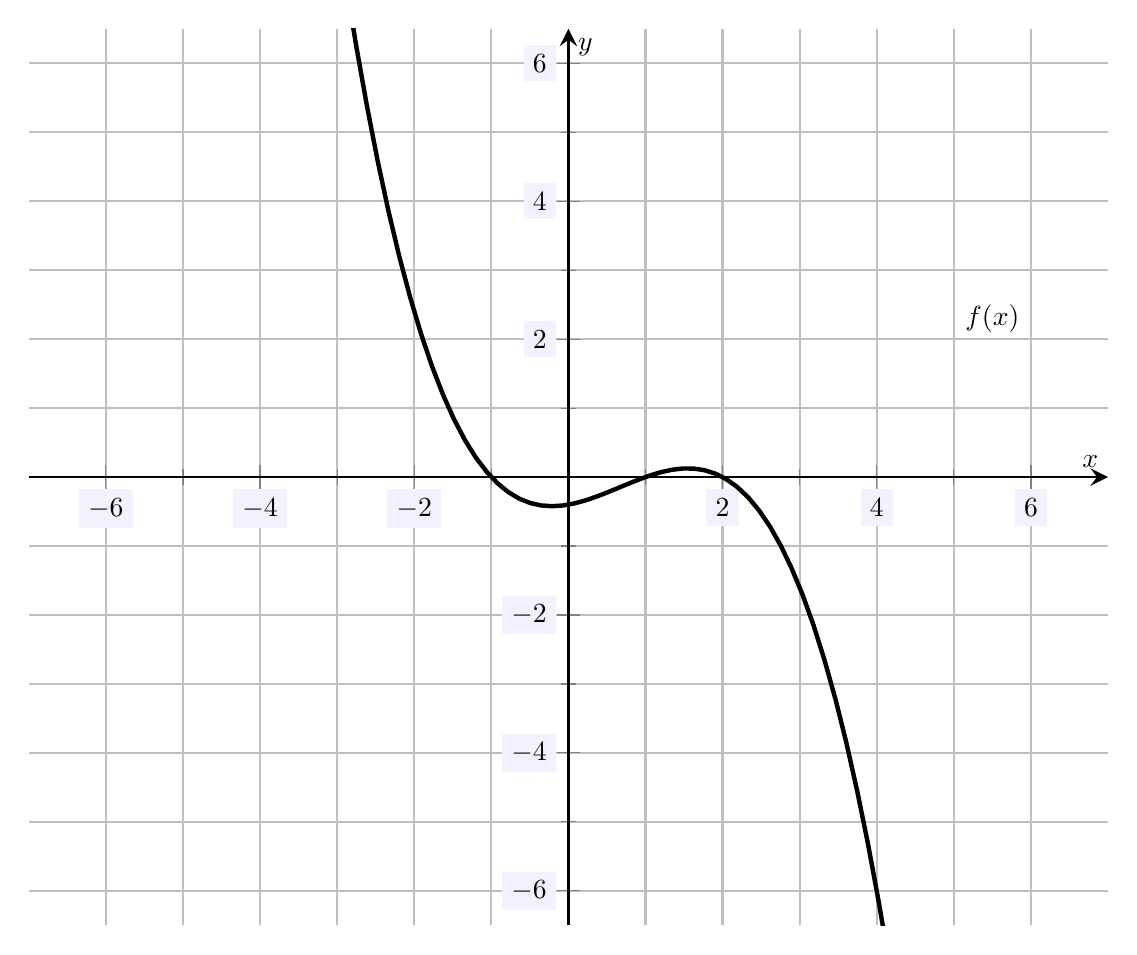
\begin{tikzpicture}[scale=2,every node/.style={scale=0.5}]
	\begin{axis}[
	grid=both,
	axis lines=middle,
	ticklabel style={fill=blue!5!white},
	xmin= -7, xmax=7,
	ymin= -6.5, ymax=6.5,
	xtick={-6,-4,-2,0,2,4,6},
	ytick={-6,-4,-2,0,2,4,6},
	minor tick = {-5,-3,...,5},
	xlabel=\(x\),ylabel=\(y\),
	]
	\node at (5.5,2.3) {$f(x)$};
	\addplot[thick, domain= -7:7, samples=100] ({x},{-1/5*(x + 1)*(x - 2)*(x -1)});
	\end{axis}
	\end{tikzpicture}
	}
	\]



\newpage



% Problem 6
\problem{10} Determine whether the point $(3, -4)$ is on the graph of $f(x)= \dfrac{x + 1}{x - 4}$. Determine also whether the point $(9, -2)$ is on the graph of $f(x)$. For each, explain why or why not. 



\newpage



% Problem 7
\problem{10} On the plot below and as accurately as possible, sketch the function $f(x)= \dfrac{2x^2 - 5}{x + 11}$. 
	\[
	\fbox{
	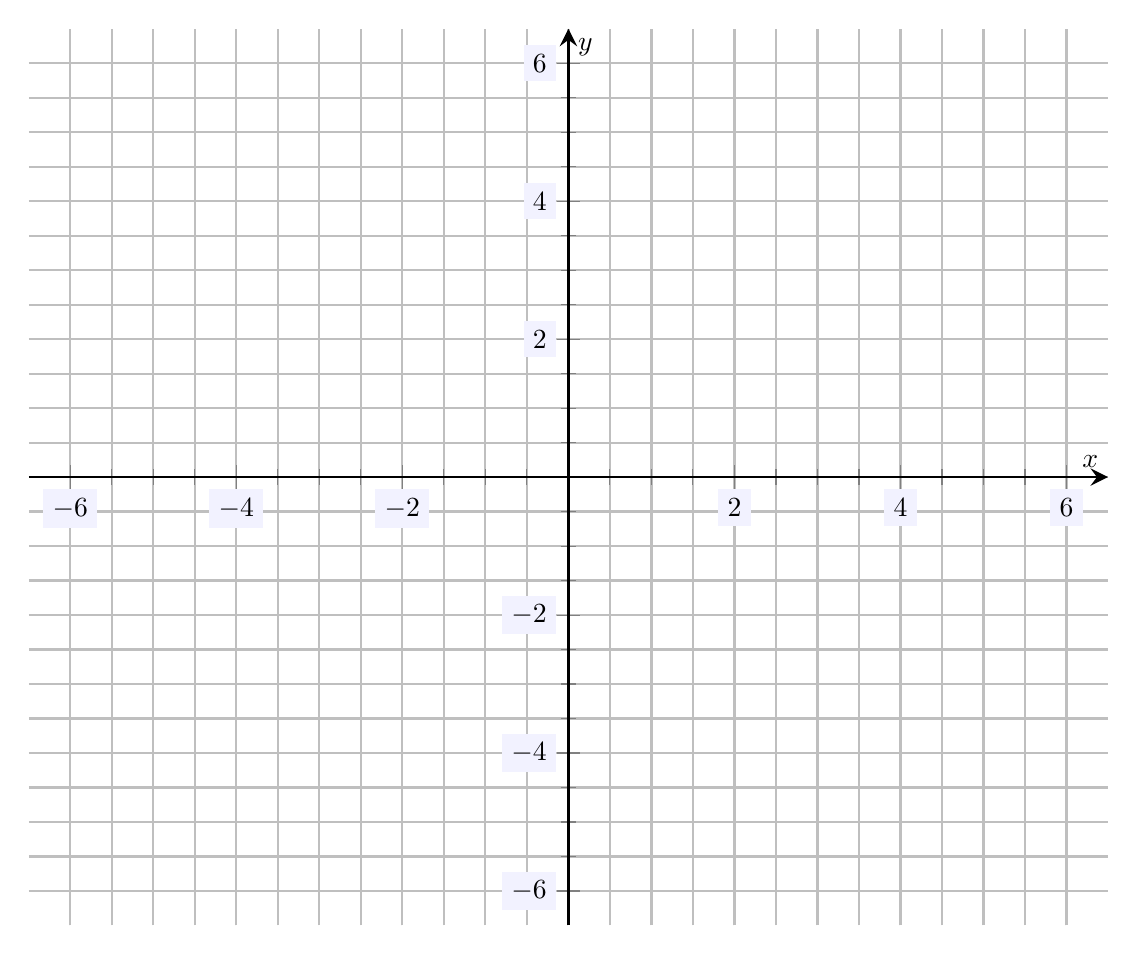
\begin{tikzpicture}[scale=2,every node/.style={scale=0.5}]
	\begin{axis}[
	grid=both,
	axis lines=middle,
	ticklabel style={fill=blue!5!white},
	xmin= -6.5, xmax=6.5,
	ymin= -6.5, ymax=6.5,
	xtick={-6,-4,-2,0,2,4,6},
	ytick={-6,-4,-2,0,2,4,6},
	minor tick = {-6,-5.5,-5,...,6},
	xlabel=\(x\),ylabel=\(y\),
	]
	\end{axis}
	\end{tikzpicture}
	}
	\] 



\newpage



% Problem 8
\problem{10} Explain why the function sketched below has an inverse and then sketch its inverse. 
	\[
	\fbox{
	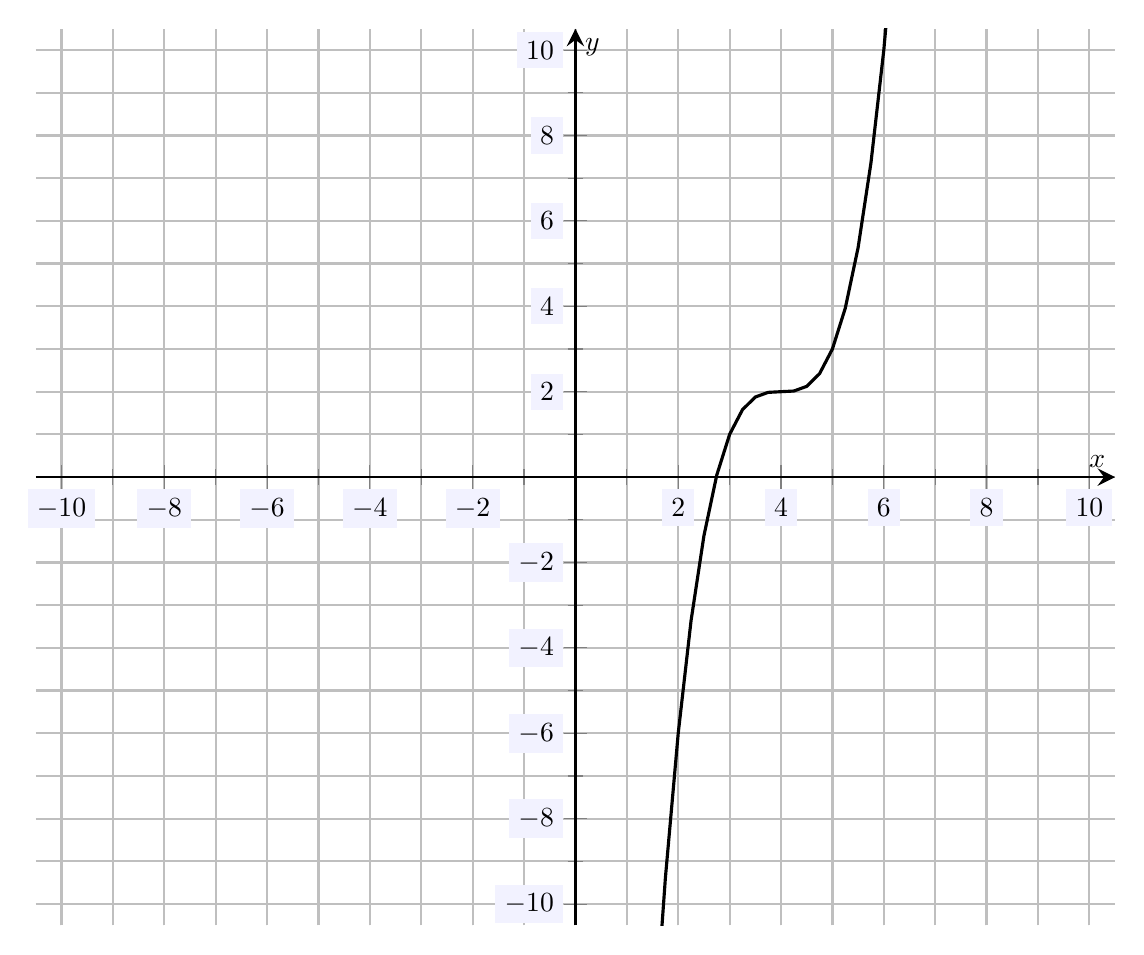
\begin{tikzpicture}[scale=2,every node/.style={scale=0.5}]
	\begin{axis}[
	grid=both,
	axis lines=middle,
	ticklabel style={fill=blue!5!white},
	xmin= -10.5, xmax=10.5,
	ymin= -10.5, ymax=10.5,
	xtick={-10,-8,-6,-4,-2,0,2,4,6,8,10},
	ytick={-10,-8,-6,-4,-2,0,2,4,6,8,10},
	minor tick = {-10,-9,...,10},
	xlabel=\(x\),ylabel=\(y\),
	]
	\addplot[line width= 0.02cm,domain= 1:7] ({x},{(x - 4)^3 + 2}); 
	\end{axis}
	\end{tikzpicture}
	}
	\] 



\newpage



% Problem 9
\problem{10} How many $y$-intercepts can a function have? Explain. Is this the same for $x$-intercepts? Explain. 



\newpage



% Problem 10
\problem{10} Using the concept of range and the fact that every non-horizontal line $\ell(x)$ intersects any horizontal line, explain why the equation $\ell(x)= c$ has a solution for every real number $c$. 


\end{document}